\documentclass[12pt]{article}
\usepackage[utf8]{inputenc}
\usepackage{graphicx}
 \usepackage{gensymb}
 \usepackage{amsmath}
\title{Photon Counting \& the Statistics of Light}
\author{Jung Lin (Doris) Lee\\ Group partners: Jennifer Ito, Manuel Silvia}
\date{\today}
\begin{document}
\maketitle
\begin{abstract}
abstract here
\end{abstract}
\section{Introduction\label{intro}}
\indent Photon statistics are the fundamental basis to optical astronomy since they constitute the data we collect in optical astronomy. 
are important to astronomy because 
optical astronomy 
galaxy morphology, 
Large sky surveys such as the Sloan Digital Sky Survey(SDSS; York et al.) and the Dark Energy Survey (DES; The Dark Energy Collaboration) imaging data in the optical wavelength.
\indent In this experiment, we recorded the arrival of photons from an LED and analyze
 In section 2, I will describe the experimental method that my group used to take the data and the results that we obtained. Subsequently, section 3 introduces the various statistical measures that we can use to describe the findings and observation on  a single dataset, including the effect of binning the data into histograms. Section 4 describes the two probability density functions that are relevant to these histograms and dataset.
\section{Experiments\label{experiment}}
	\subsection{Methods}
\indent The arrival of a photon is registered by the photomultiplier tube (PMT), and data was acquired using the CoinPro software. The resulting processed data file is a series of time stamps of when the data arrived. Since CoinPro is ran on a 32-bit machine, we can see the cycling through of time in FIG REF. Although absolute time stamp is the recorded quantity, it is often more useful to consider the time elapsed between two consecutive events ($\texttt{dt}$) as plotted in Fig. in order to get a sense of  the photon arrival rate for some sample waiting time.
\begin{figure}[h]
\centering
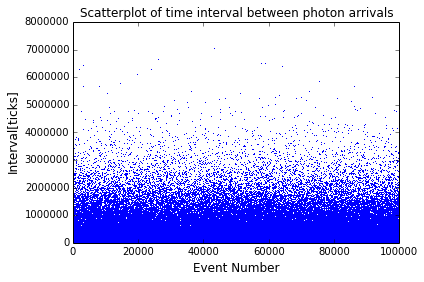
\includegraphics[width=1\textwidth]{figures/interval_scatterplot}
\caption{With the removal of after pulse event, we can see that there is a decline in the number of events. This makes sense because we are doing an interval cut at 3000 clock ticks, which should result in a clear boundary at y=3000 but this can not be seen due to the large range of interval value that the y-axis spans over. The data representation in Fig. \ref{fitted_histo_gate_or_no} better shows the the effect of gating afterpulses. }
\label{scatterplot}
\end{figure}
\\
\indent Sometimes noise pulses resembling Fig.\ref{afterpulse} can be observed after the original pulse. These events are caused by  the ionization of residual gas molecules in the PMT's vacuum chamber.  We eliminate this systematic effects by cutting away data with subsequent pulses lie within the time frame of 2.5$\mu$s  after an original pulse as shown in Fig.\ref{fitted_histo_gate_or_no}.

\begin{figure}[h]
\centering
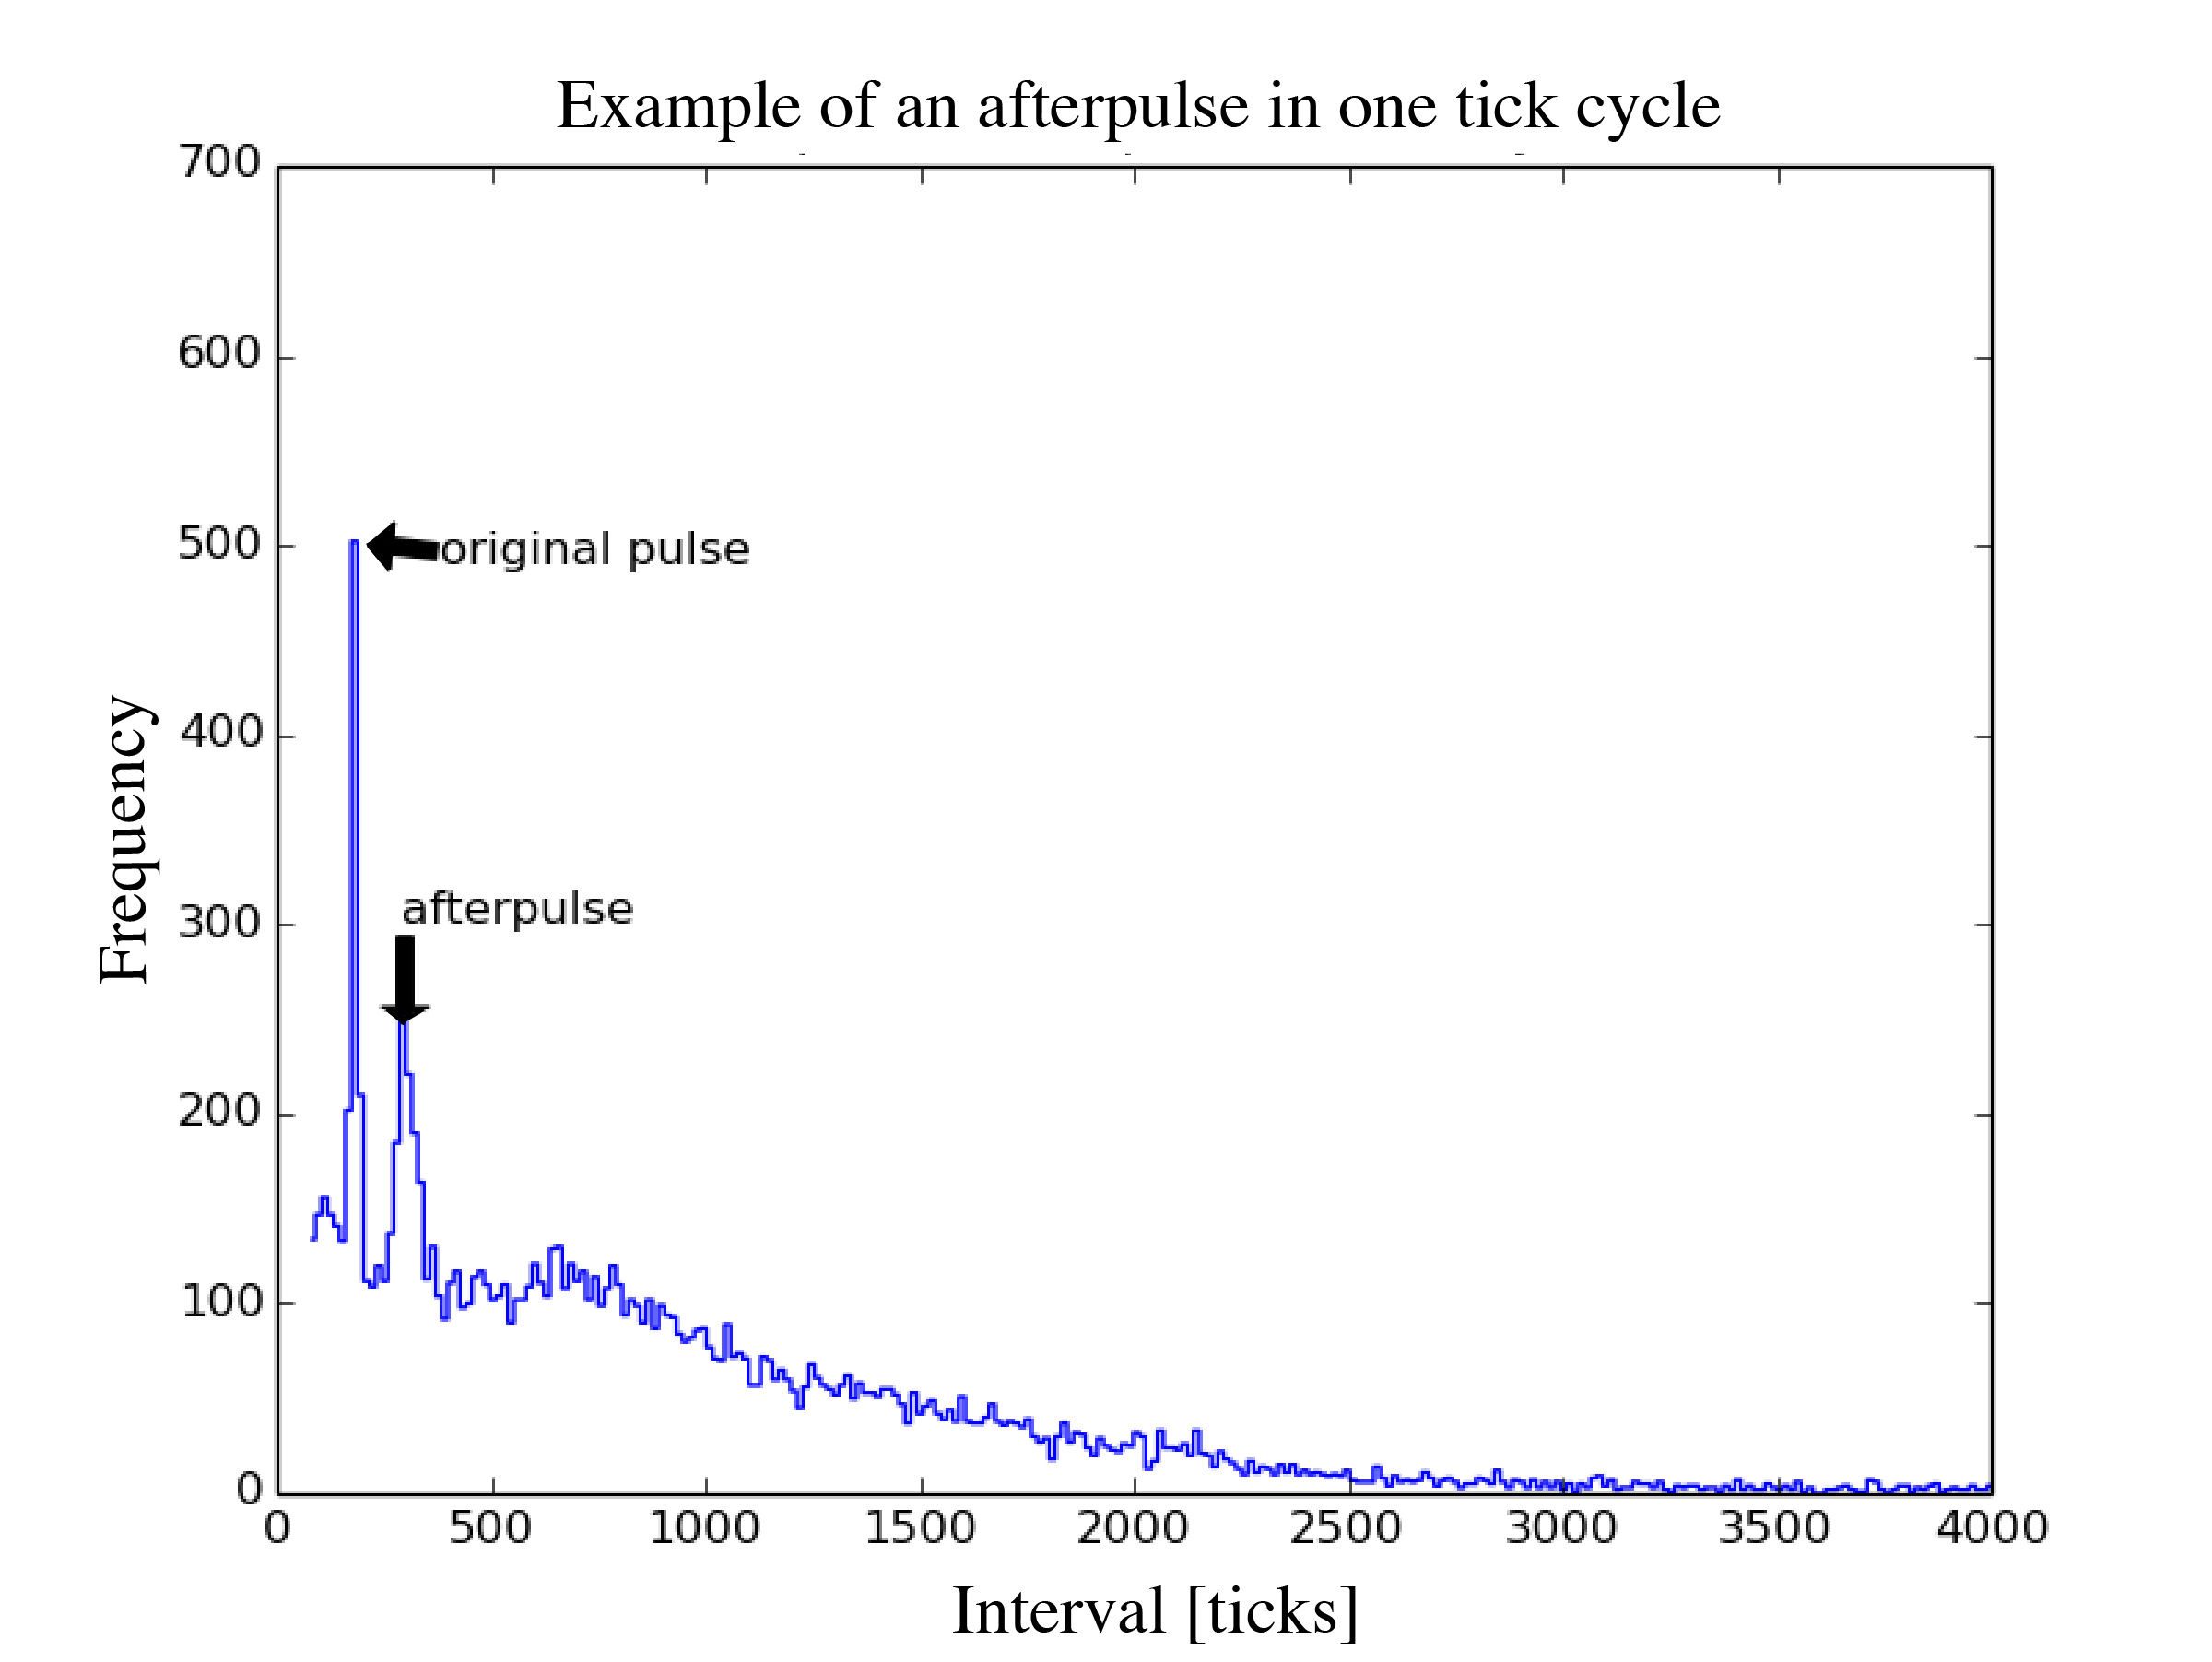
\includegraphics[width=1\textwidth]{figures/afterpulse}
\caption{With histogram of bin size = 500,000, the two peaks (original and afterpulse) as well as a gradual decline of ticks in the next \~3000 clock ticks can be seen here.}
\label{afterpulse}
\end{figure}
   \subsection{Changing LED Brightness}
\indent By listening to ticks on the squawker, there was no detectable difference from the 3 o'clock off position to the 12 o'clock position. Therefore, we started off at the 12 o'clock location and went to the max location ($\approx$90\degree), diving this region into 6 equal parts \footnote{Although it seems like only 5 data points are shown in the plot, this is merely an artifact of the choice of data representation as circles as  the first two data points lie so closely that they are almost indistinguishable. This is easily verified by using the dot representation with \texttt{matplotlib's} `,`setting} is roughly 15\degree  increments. Even though the measurement of the LED brightness is eyeballed and not that precise, it did not significantly affect the plot since the relation is linear . No matter what the brightness is, in theory, the data point should always follow the slope =1 linear relation.
\begin{figure}[h]
\centering
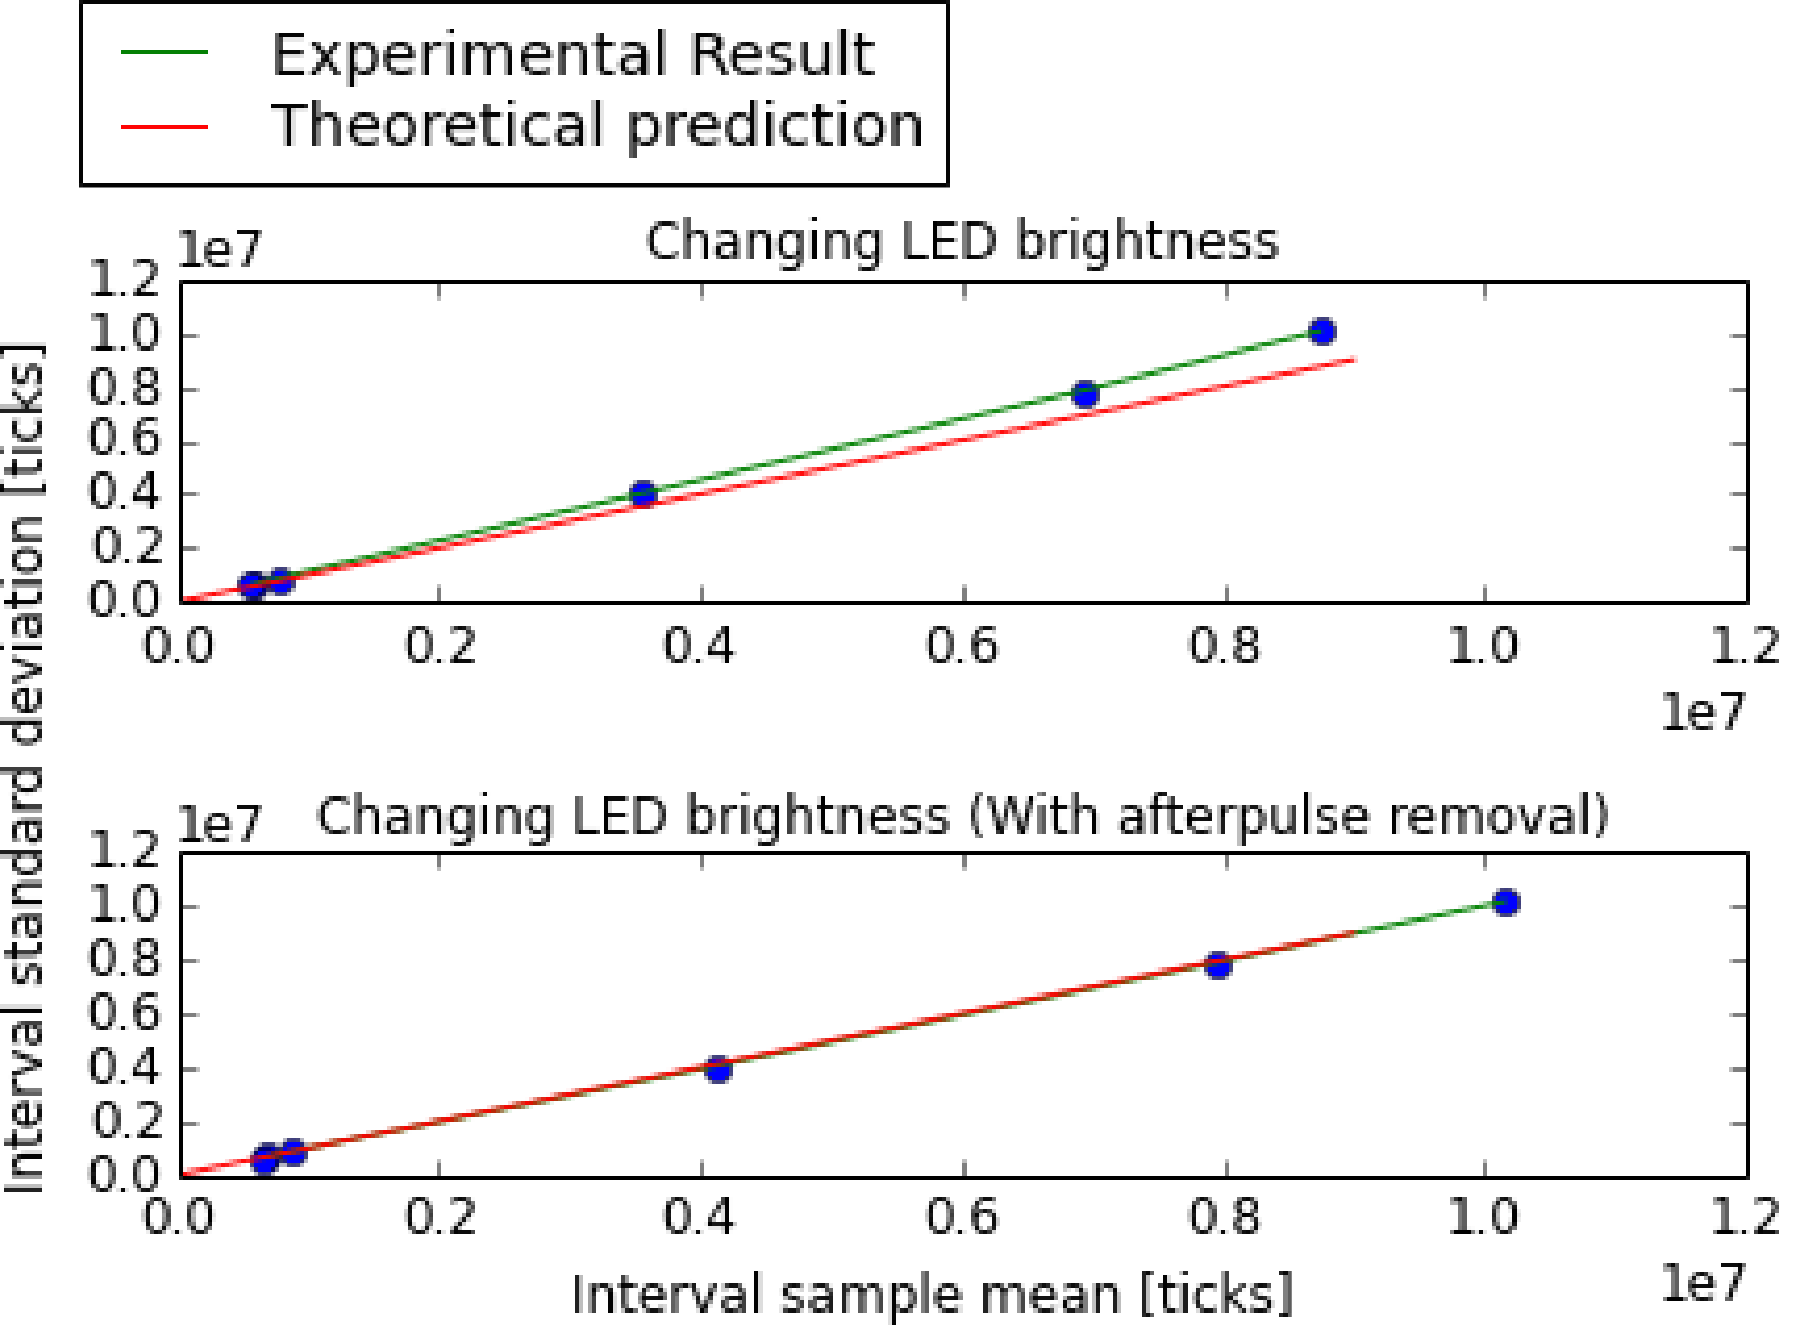
\includegraphics[width=0.8\textwidth]{figures/changeLED}
\caption{Showing linear relation between standard deviation and sample mean. The slope of the line should one since both the standard deviation and the sample mean of each dataset is equal to the single-parameter that governs the behavior of the exponential distribution.}
\label{changeLED}
\end{figure}
\section{Descriptive Statistics and Histograms\label{stats}}
Since the Poisson distributuon is discrete, the mean converges to the expected value ad the number of trials(N) is large. In Fig. we take 
\section{Photon Statistics\label{pstats}}

 	\subsection{Exponential Distribution}
 	Exponential distribution described by Eq.\ref{exp_distr} governs the histogram of $\texttt{dt}$, the elapsed time between photon arrival event.
\begin{equation} \label{exp_distr}
 P(t,\tau)=\frac{1}{\tau}e^{-\frac{t}{\tau}}
\end{equation}
 	 A defining characteristic of the exponential distribution is that it is continous``memorylessness``. In this case, the photon arrival rate at some moment in time,t, is not dependent on the photon arrival rate prior to time t.  The green curve in Fig.\ref{fitted_histo_gate_or_no} is the plotted from the analytical solution shown in Eq.\ref{int_exp}, which is obtained from integrating the exponential distribution with a step-size $\Delta t =1.42x10^7$and  $\tau$ set as the mean of the $\texttt{dt}$ dataset .  
 	 \begin{equation}\label{int_exp}
 	 \int^{t+\Delta t}_\tau\frac{1}{\tau}e^\frac{t}{\tau}dt=-e^\frac{t+\Delta t}{\tau}+e^\frac{t}{\tau}
	\end{equation} 	  
Since the exponential distribution is a unity-normalized PDF, this result is scaled by the number of events to fit the histogram.
 	\begin{figure}[h]
		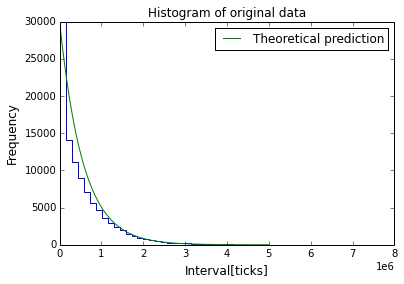
\includegraphics[width=0.5\textwidth]{figures/fitted_histo}
		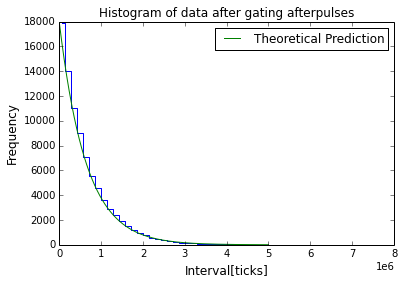
\includegraphics[width=0.5\textwidth]{figures/fitted_histo_with_gating}
		\caption{Histogram of bin size = 50 before (left) and after (right) cutting away the afterpulses.}
		\label{fitted_histo_gate_or_no}
	\end{figure}
 	\subsection{Poisson Distribution}
 	Although closely-related, the Poisson distribution is unlike the exponential distribution in that it is a discrete probability distribution that arises from measuring the number of events that occur within a fixed sampling interval . The underlying process is the same (rare event for very large N) but the experiment method is different. In this case, the experiment is the same, but we change the way the data is represented, as binned data for a fixed bin size. 
 	 	\begin{figure}[h]
		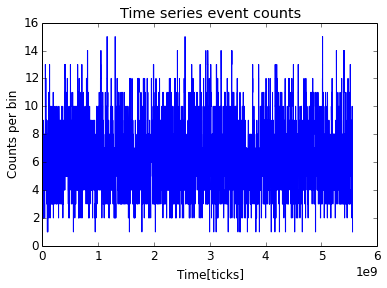
\includegraphics[width=0.5\textwidth]{figures/time_series}
		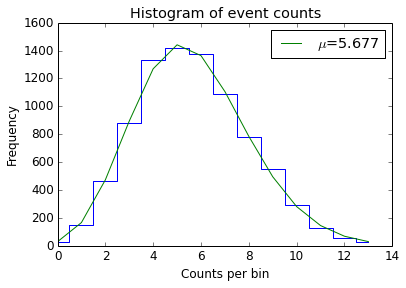
\includegraphics[width=0.5\textwidth]{figures/poisson_histo}
		\caption{By using a Poisson curve fit, we find that the $\mu$ is 5.677.}
		\label{poisson}
	\end{figure}
\section{Conclusion\label{end}}
In this lab, we 
Possible extensions to this project is to investigate 
\end{document}
